\documentclass[margin = 1cm]{standalone}
\usepackage{tikz}
\usepackage{amssymb}
\usetikzlibrary{shapes.geometric,arrows.meta}
\tikzset{one/.style={draw,minimum width = 8em,align = center,inner xsep = .7cm,inner ysep = .4cm},
two/.style={shape aspect=4,diamond,draw,align = center},
three/.style={trapezium, draw,trapezium left angle=60, trapezium right angle=120,minimum width = 16em,align = center,inner ysep = 8pt},
arrow/.style = {-{Triangle[scale = 1]},thick}}

\begin{document}
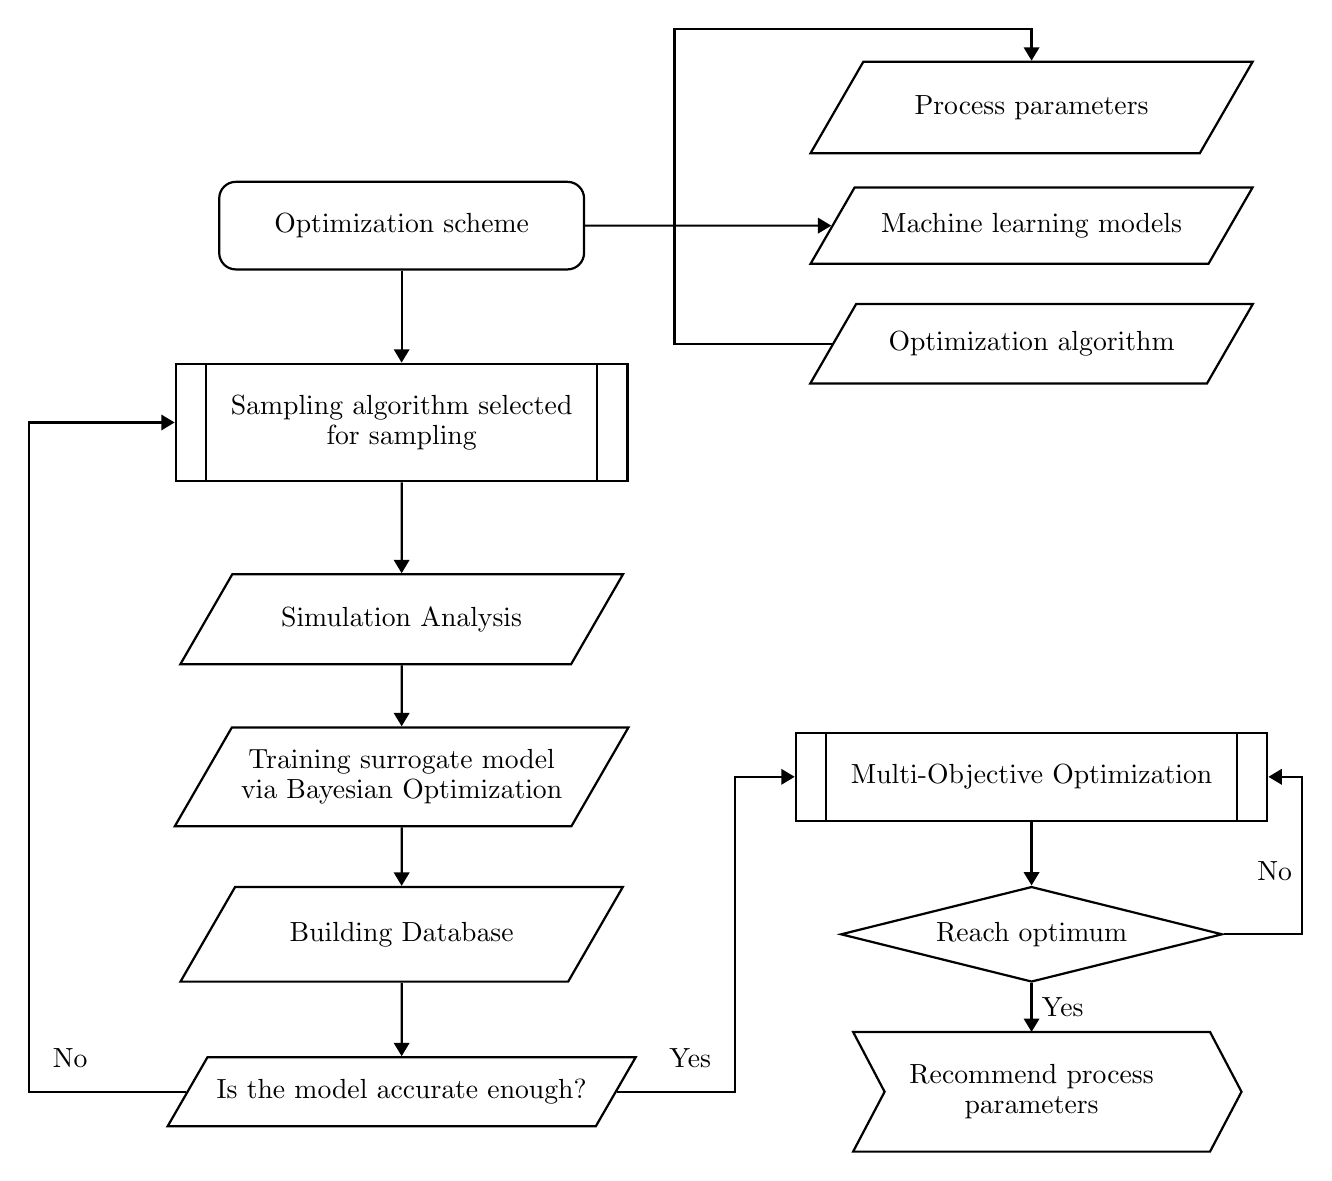
\begin{tikzpicture}[thick]
\linespread{.9}
\node[one,rounded corners = 6pt] (a) at (0,0) {Optimization scheme}; 
\node[one,] (b) at (0,-2.5) {Sampling algorithm selected \\ for sampling};
\draw[] ([xshift = .4cm]b.south west) -- ([xshift = .4cm]b.north west);
\draw[] ([xshift = -.4cm]b.south east) -- ([xshift = -.4cm]b.north east);
\node[three] (c) at (0,-5) {Simulation Analysis};
\node[three] (d) at (0,-7) {Training surrogate model \\ via Bayesian Optimization};
\node[three] (e) at (0,-9) {Building Database};
\node[three] (f) at (0,-11) {Is the model accurate enough?};

\node[one] (g) at (8,-7) {Multi-Objective Optimization};
\draw[] ([xshift = .4cm]g.south west) -- ([xshift = .4cm]g.north west);
\draw[] ([xshift = -.4cm]g.south east) -- ([xshift = -.4cm]g.north east);
\node[two] (h) at (8,-9) {Reach optimum};
\node[one,draw=none] (i) at (8,-11) {Recommend process \\ parameters};
\draw[] ([xshift = .4cm]i.west) -- (i.north west) -- (i.north east) -- ([xshift = .4cm]i.east) -- (i.south east) -- (i.south west) -- cycle;

\node[three] (j) at (8,1.5) {Process parameters};
\node[three] (k) at (8,0) {Machine learning models};
\node[three] (l) at (8,-1.5) {Optimization algorithm};

\draw[arrow] (a) -- (b);
\draw[arrow] (b) -- (c);
\draw[arrow] (c) -- (d);
\draw[arrow] (d) -- (e);
\draw[arrow] (e) -- (f);

\draw[arrow] (g) -- (h);
\draw[arrow] (h) -- (i)node[pos=0.5,right] {Yes};

\draw[arrow] (a) -- (k);

\draw[arrow] (l.west) --++ (-2,0) -- ++ (0,4) -| (j); 

\draw[arrow] (f.west) --++ (-2,0) |- (b)node[pos=0,above right = 5pt] {No};
\draw[arrow] (h.east) --++ (1,0) |- (g)node[pos=0.2,left] {No};

\draw[arrow] (f.east) --++ (1.5,0) |- (g)node[pos=0,above left = 5pt] {Yes};
\end{tikzpicture}
\end{document}